\documentclass[12pt,a4paper]{article}

\usepackage[margin=2.5cm]{geometry}
\usepackage[utf8]{inputenc}
\usepackage[brazil]{babel}
\usepackage{lmodern}
\usepackage{fancyhdr}
\usepackage{tocloft}
\usepackage{amsmath}
\usepackage{graphicx}
\usepackage{booktabs}
\usepackage{array}
\usepackage{float}
\usepackage{hyperref}
\usepackage{lastpage}
\usepackage{subcaption}
\usepackage{multirow}

\graphicspath{{../../../imagens_gerais/} {images/}} 

\pagestyle{fancy}
\fancyhf{} 
\setlength{\headheight}{30pt}
\lhead{
  \includegraphics[height=1.2cm]{lafe_logo_ingles.jpg} \\
  \small
  Doc ID: PLT0075 \quad
  Doc tipo: Relatório de fabricação \quad
}
\rhead{
  \small \textbf{PLT0075 Suspended core em PETG esverdeado} \\
  Page \thepage\ of \pageref{LastPage}
}
\lfoot{\small \textcopyright\ 2026 LaFE. All rights reserved.}
\rfoot{\small Última data de revisão: 17/07/2026}

\begin{document}

  Descrição da participação dos envolvidos na fabricação desta fibra:
  \begin{itemize}
    \item Ivan Prearo: Fabricação e puxamento
    \item Gustavo Freitas: puxamento
  \end{itemize}

  \section*{Puxamento}
  \label{sec:puxamento}

Este puxamento é de uma preforma do tipo \textit{staircase-core}.
A preforma tem 100mm de comprimento útil e é mostrada na Figura \ref{fig:foto_preforma}, e tem microestrutura \textit{hollow-core} da Figura \ref{fig:desenho_preforma}.
As dimensões são mostradas na Tabela \ref{tab:medidas_preforma}, com a identificação de cada dimensão mostrada na Fig \ref{fig:secoes}.

  \begin{table}[H]
    \centering
	  \begin{tabular}{c|ccc}	
		  \textbf{Seção de corte} & \textbf{Medida} & \textbf{Medida absoluta [mm]} & \textbf{Medida relativa} \\ 
		  \hline
		  \multirow{4}{*}{Transversal}
      & $\phi_{out}$ & 15 & 1.000 \\
		  & $L_{clad}$ & 3 & 0.200 \\
      & $\phi_{core}$ & 2.4 & 0.160 \\
		  & $L_{strut}$ & 0.55 & 0.037 \\
      \hline
      \multirow{3}{*}{Longitudinal}
      & $h_{strut}$ & 3 & 0.200 \\
      & $\delta$ & 1.1 & 0.073 \\
      & $\theta$ & 5$^\circ$ & ---
	  \end{tabular}
	  \caption{Medidas na preforma.}
	  \label{tab:medidas_preforma}
  \end{table}

\begin{figure}[H]
	\centering
  \begin{subfigure}[t]{0.8\linewidth}
    \centering
	  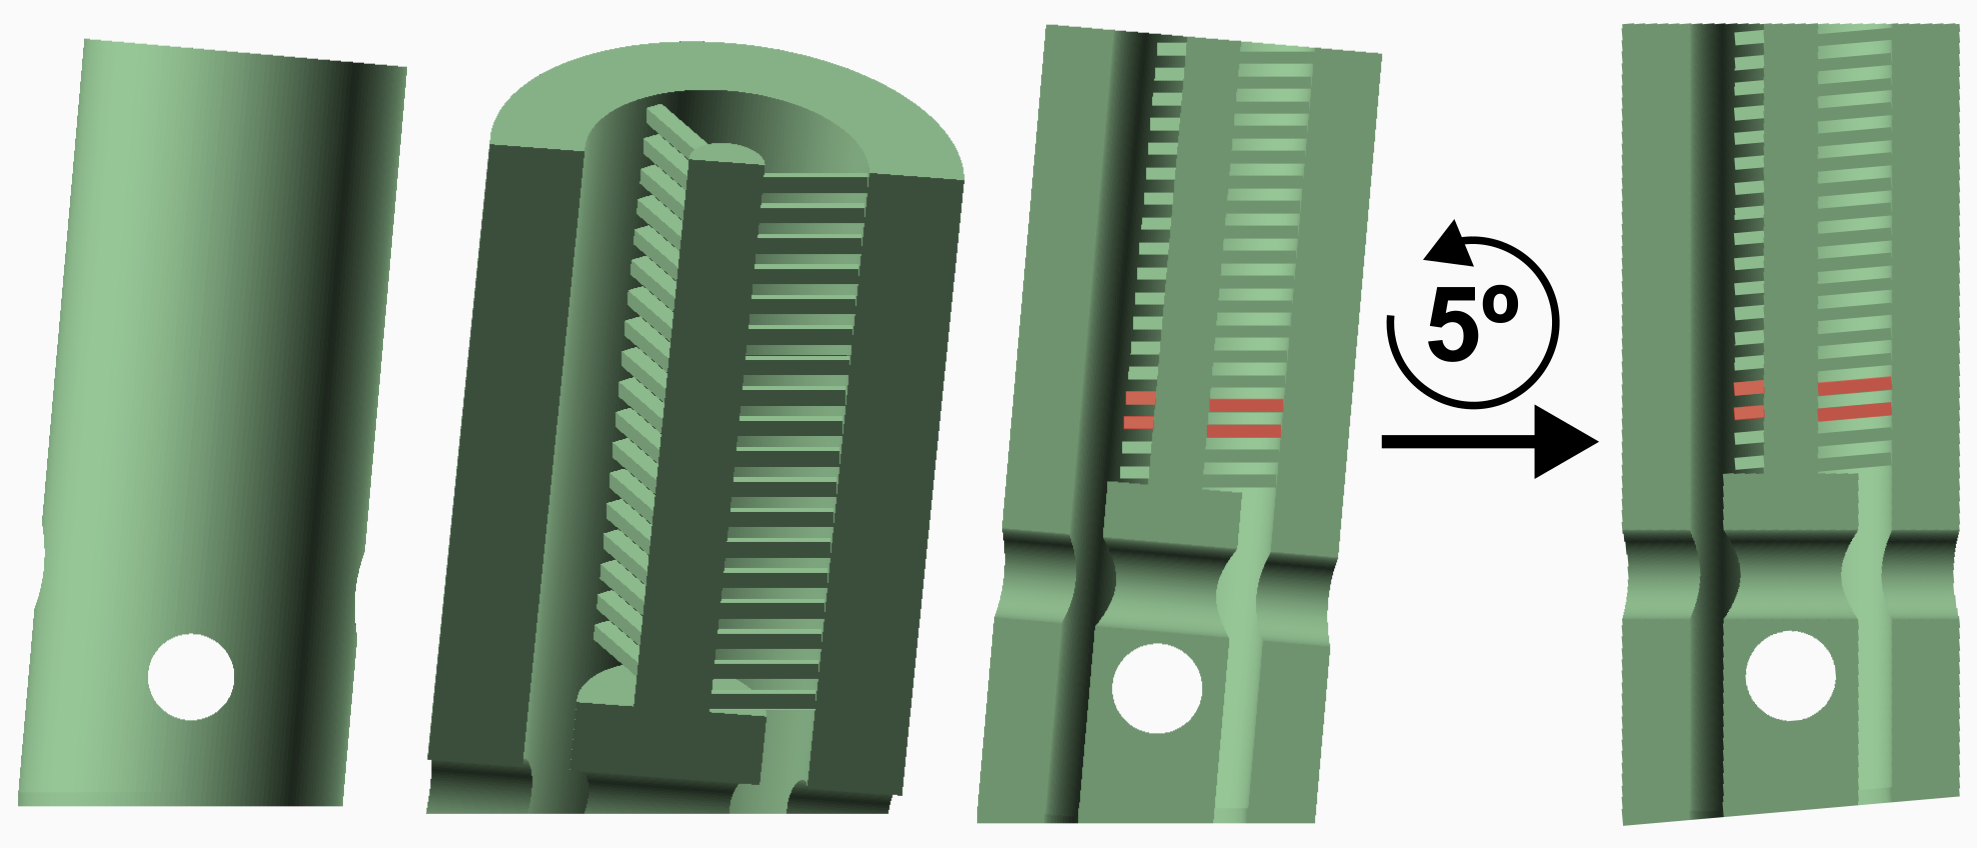
\includegraphics[width=\linewidth]{Desenhos.png}
    \caption{Seções bidimensionais da preforma.}
    \label{fig:desenho_preforma}
  \end{subfigure}
  \begin{subfigure}[t]{0.15\linewidth}
    \centering
	  
\includegraphics[height=2.3\linewidth]{Preforma.jpeg}
    \caption{Preforma.}
    \label{fig:foto_preforma}
  \end{subfigure}
	\caption{Modelo usado na fabricação da preforma puxada e foto da mesma. Desenhos em escala.}
	\label{fig:preforma}
\end{figure}

\begin{figure}[H]
  \centering
  \begin{subfigure}[t]{0.48\linewidth}
    \centering
    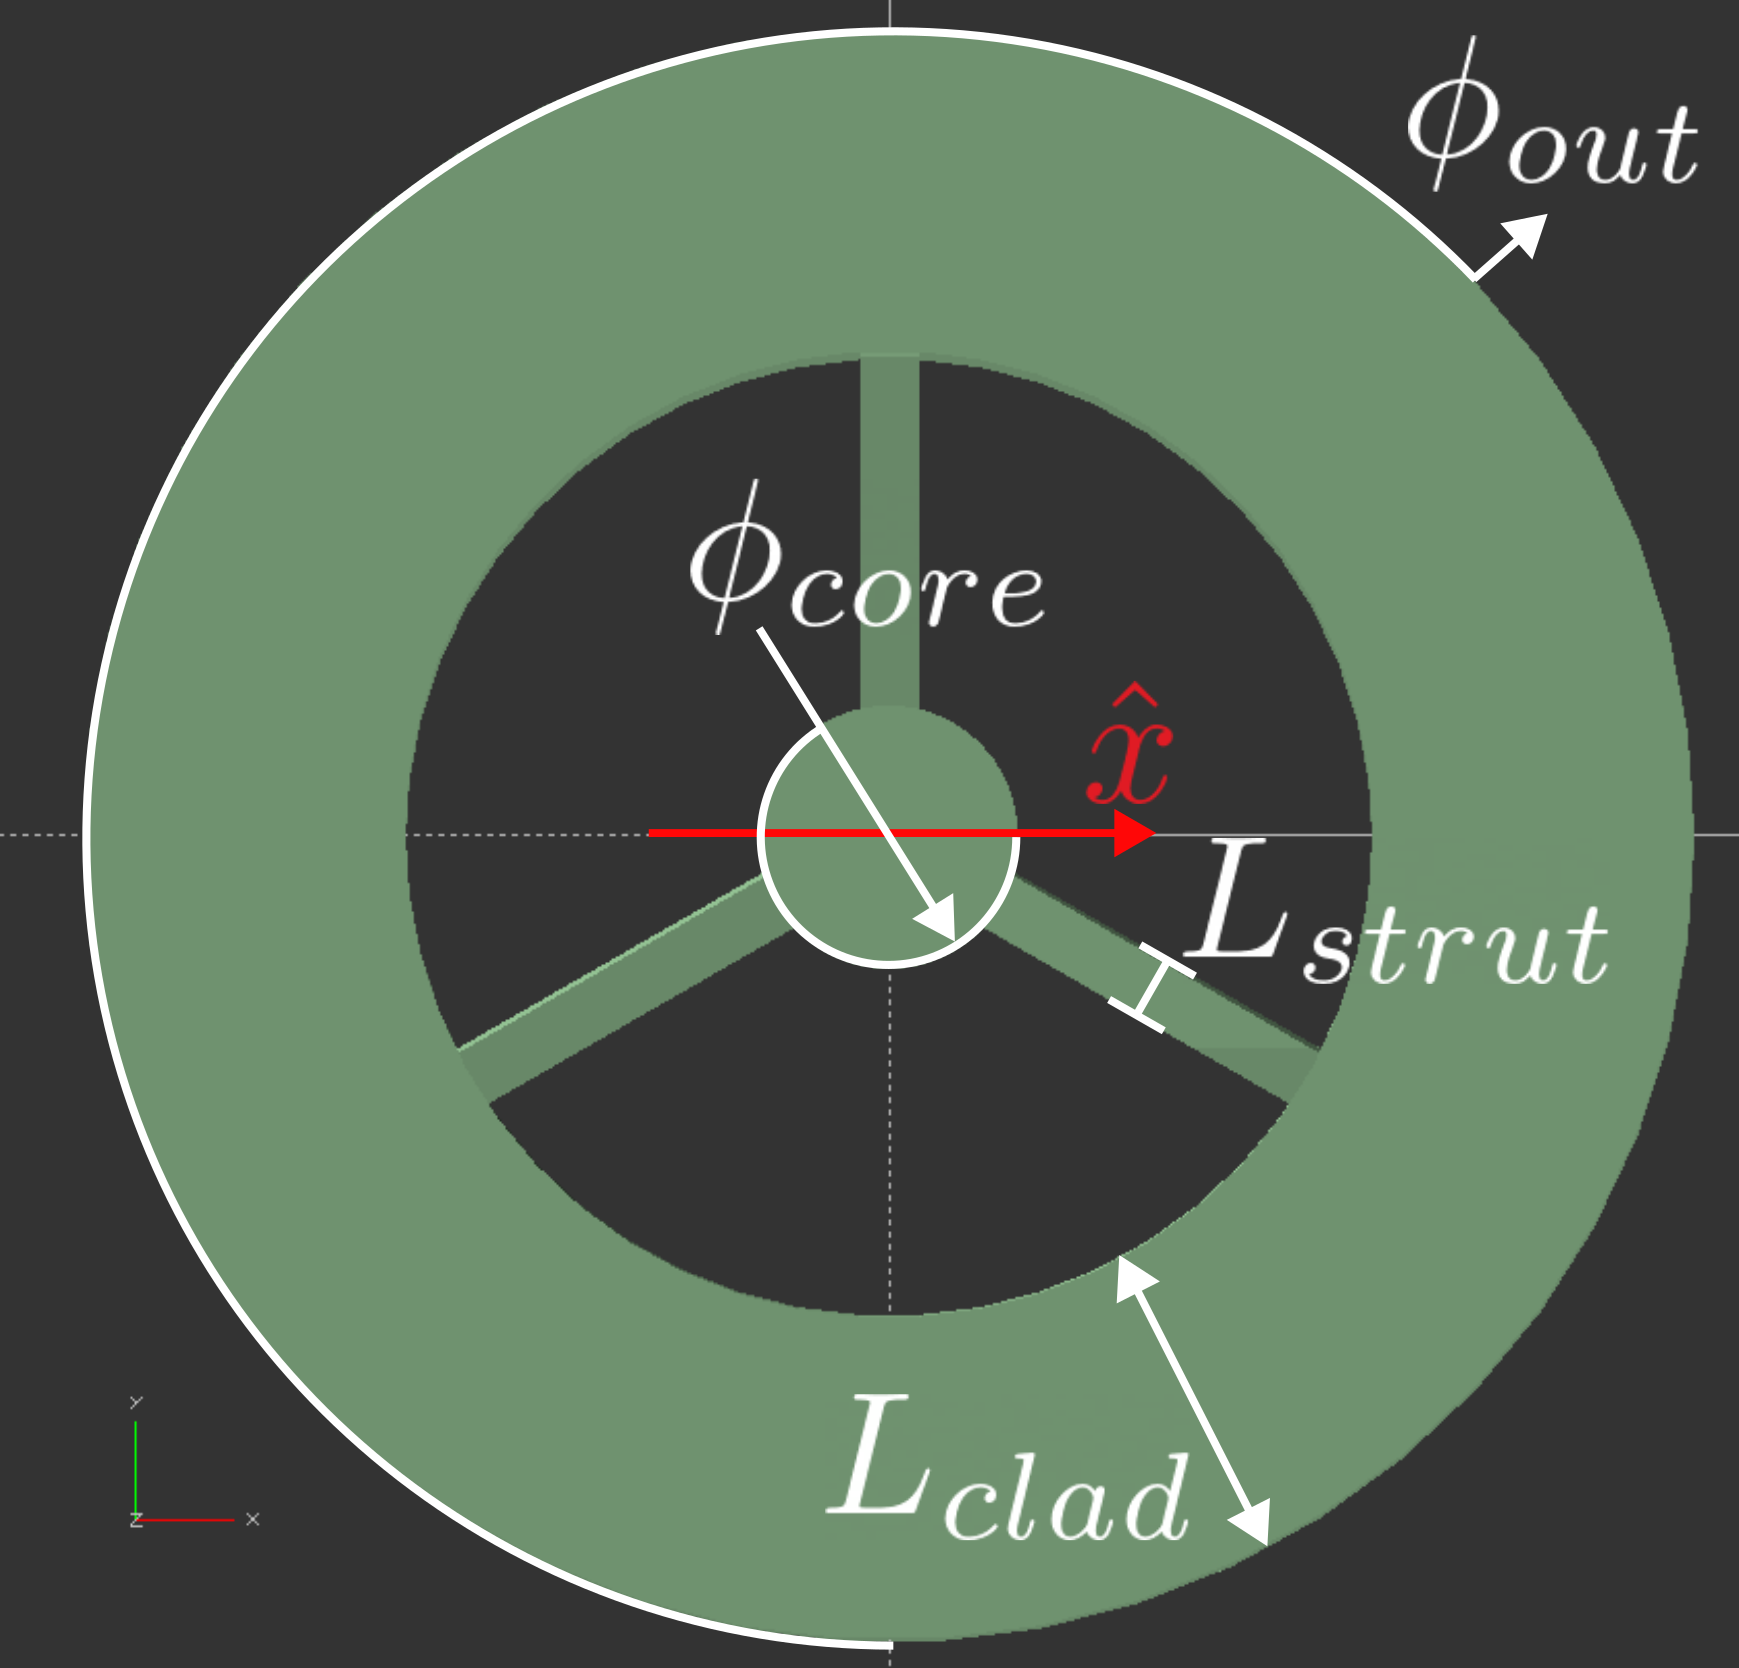
\includegraphics[width=0.74\linewidth]{plano_xy.png}
    \caption{Seção transversal.}
    \label{fig:sec_transversal}
  \end{subfigure}
  \begin{subfigure}[t]{0.48\linewidth}
    \centering
    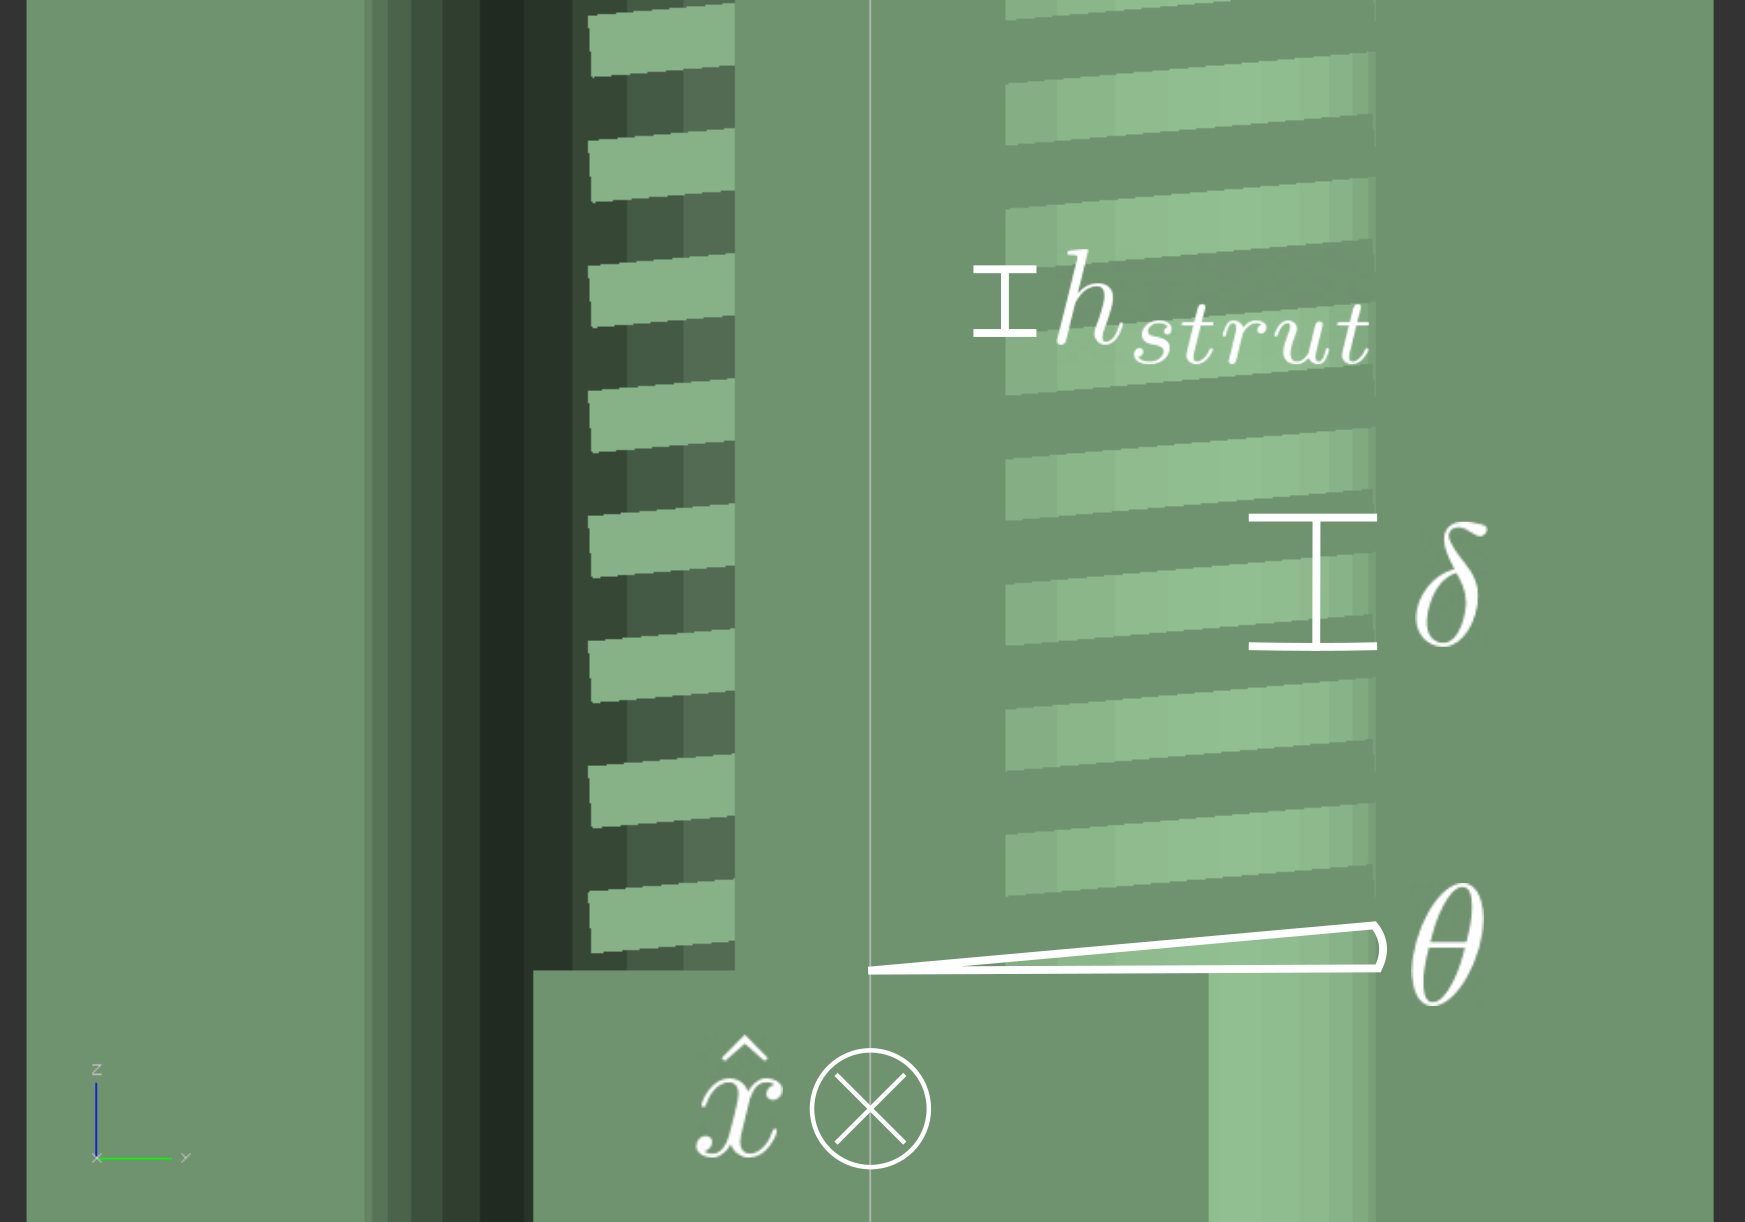
\includegraphics[width=\linewidth]{plano_yz.png}
    \caption{Seção longitudinal.}
    \label{fig:sec_longitudinal}
  \end{subfigure}
  \caption{Definições de medidas relevantes na fibra projetada. O eixo $\hat x$ é usado como eixo de rotação e o eixo $\hat z$ é na direção da fibra.}
  \label{fig:secoes}
\end{figure}


  Para realizar o puxamento utilizamos a rampa de temperatura descrita na Tabela \ref{tab:puxamento_rampa}.

\begin{table}[H]
  \centering
  \begin{tabular}{ccc}   
    \toprule 
    \textbf{Fase} & \textbf{[°C]} & \textbf{Tempo [min]} \\ 
    \midrule
    \multirow{2}{*}{Secagem} & 60 & 60 \\
                              & 80 & 20\\
    \midrule
    \multirow{2}{*}{Escoamento} & 100 & 5 \\
                              & 110 & 2 \\ 
    \midrule
    \multirow{1}{*}{Puxamento} & 120 & --- \\
    \bottomrule
  \end{tabular}
  \caption{Rampa de temperatura no forno da torre antes e durante o puxamento.}
  \label{tab:puxamento_rampa}
\end{table}

\section*{Resultados}
\label{sec:resultados}

Foram produzidos cerca de 40 metros da fibra descrita acima, com diâmetros finais entre 1mm e 200$\mu$m.
As bandas \textit{Lixo} e A têm o diâmetro mais instável, e a primeira delas os maiores diâmetros.
Juntas essas duas bandas somam cerca de 17 metros dos 40 produzidos.
As bandas B e, principalmente, C mantiveram um diâmetro mais estável durante sua produção, com máximos próximos de 400$\mu$m e mínimos de 200$\mu$m.

As medidas de cada banda estão representadas na Tabela \ref{tab:medidas_produzidas}; e os diâmetros medidos durante o puxamento estão na Fig. \ref{fig:diametros}, com anotações de começo e fim de cada banda.

\begin{figure}[H]
  \centering
  \begin{subfigure}[t]{0.9\linewidth}
    \centering
    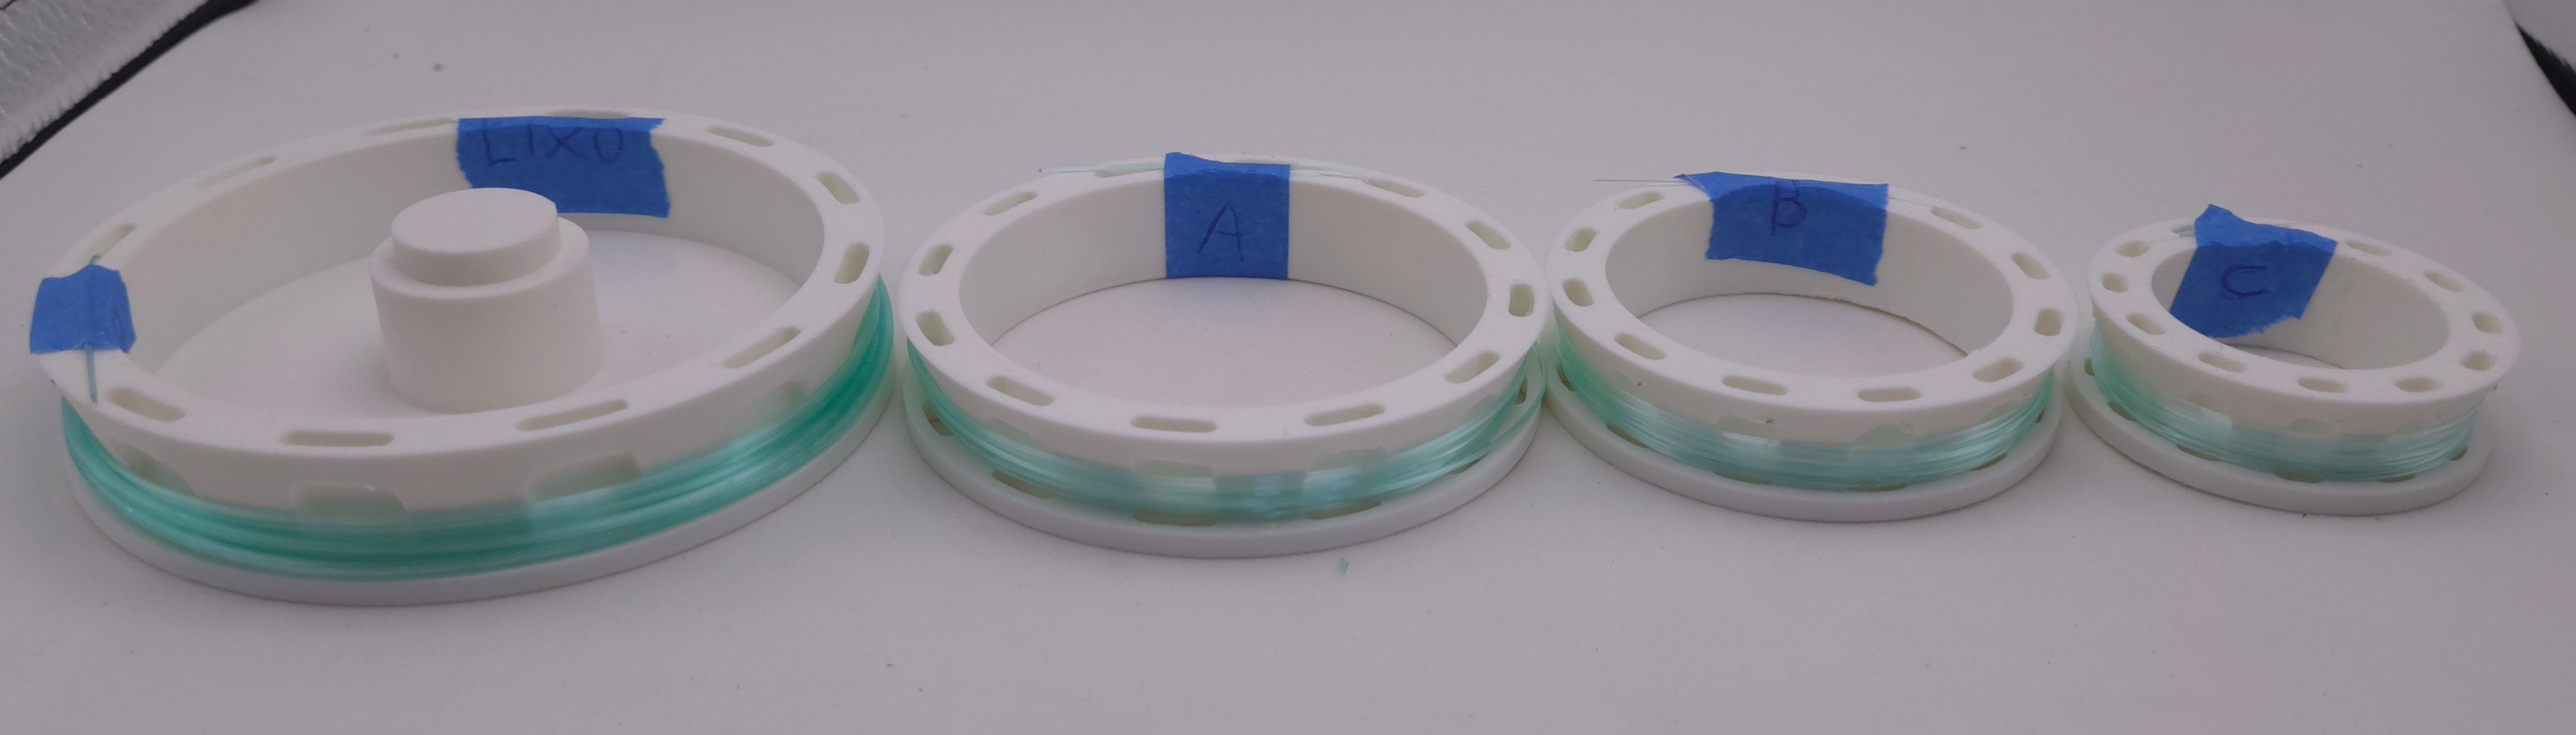
\includegraphics[width=\linewidth]{Bandas.jpg}
    \caption{Bandas produzidas no puxamento dessa amostra.}
    \label{fig:bandas_LixABC}
  \end{subfigure}
  \begin{subfigure}[t]{0.6\linewidth}
    \centering
    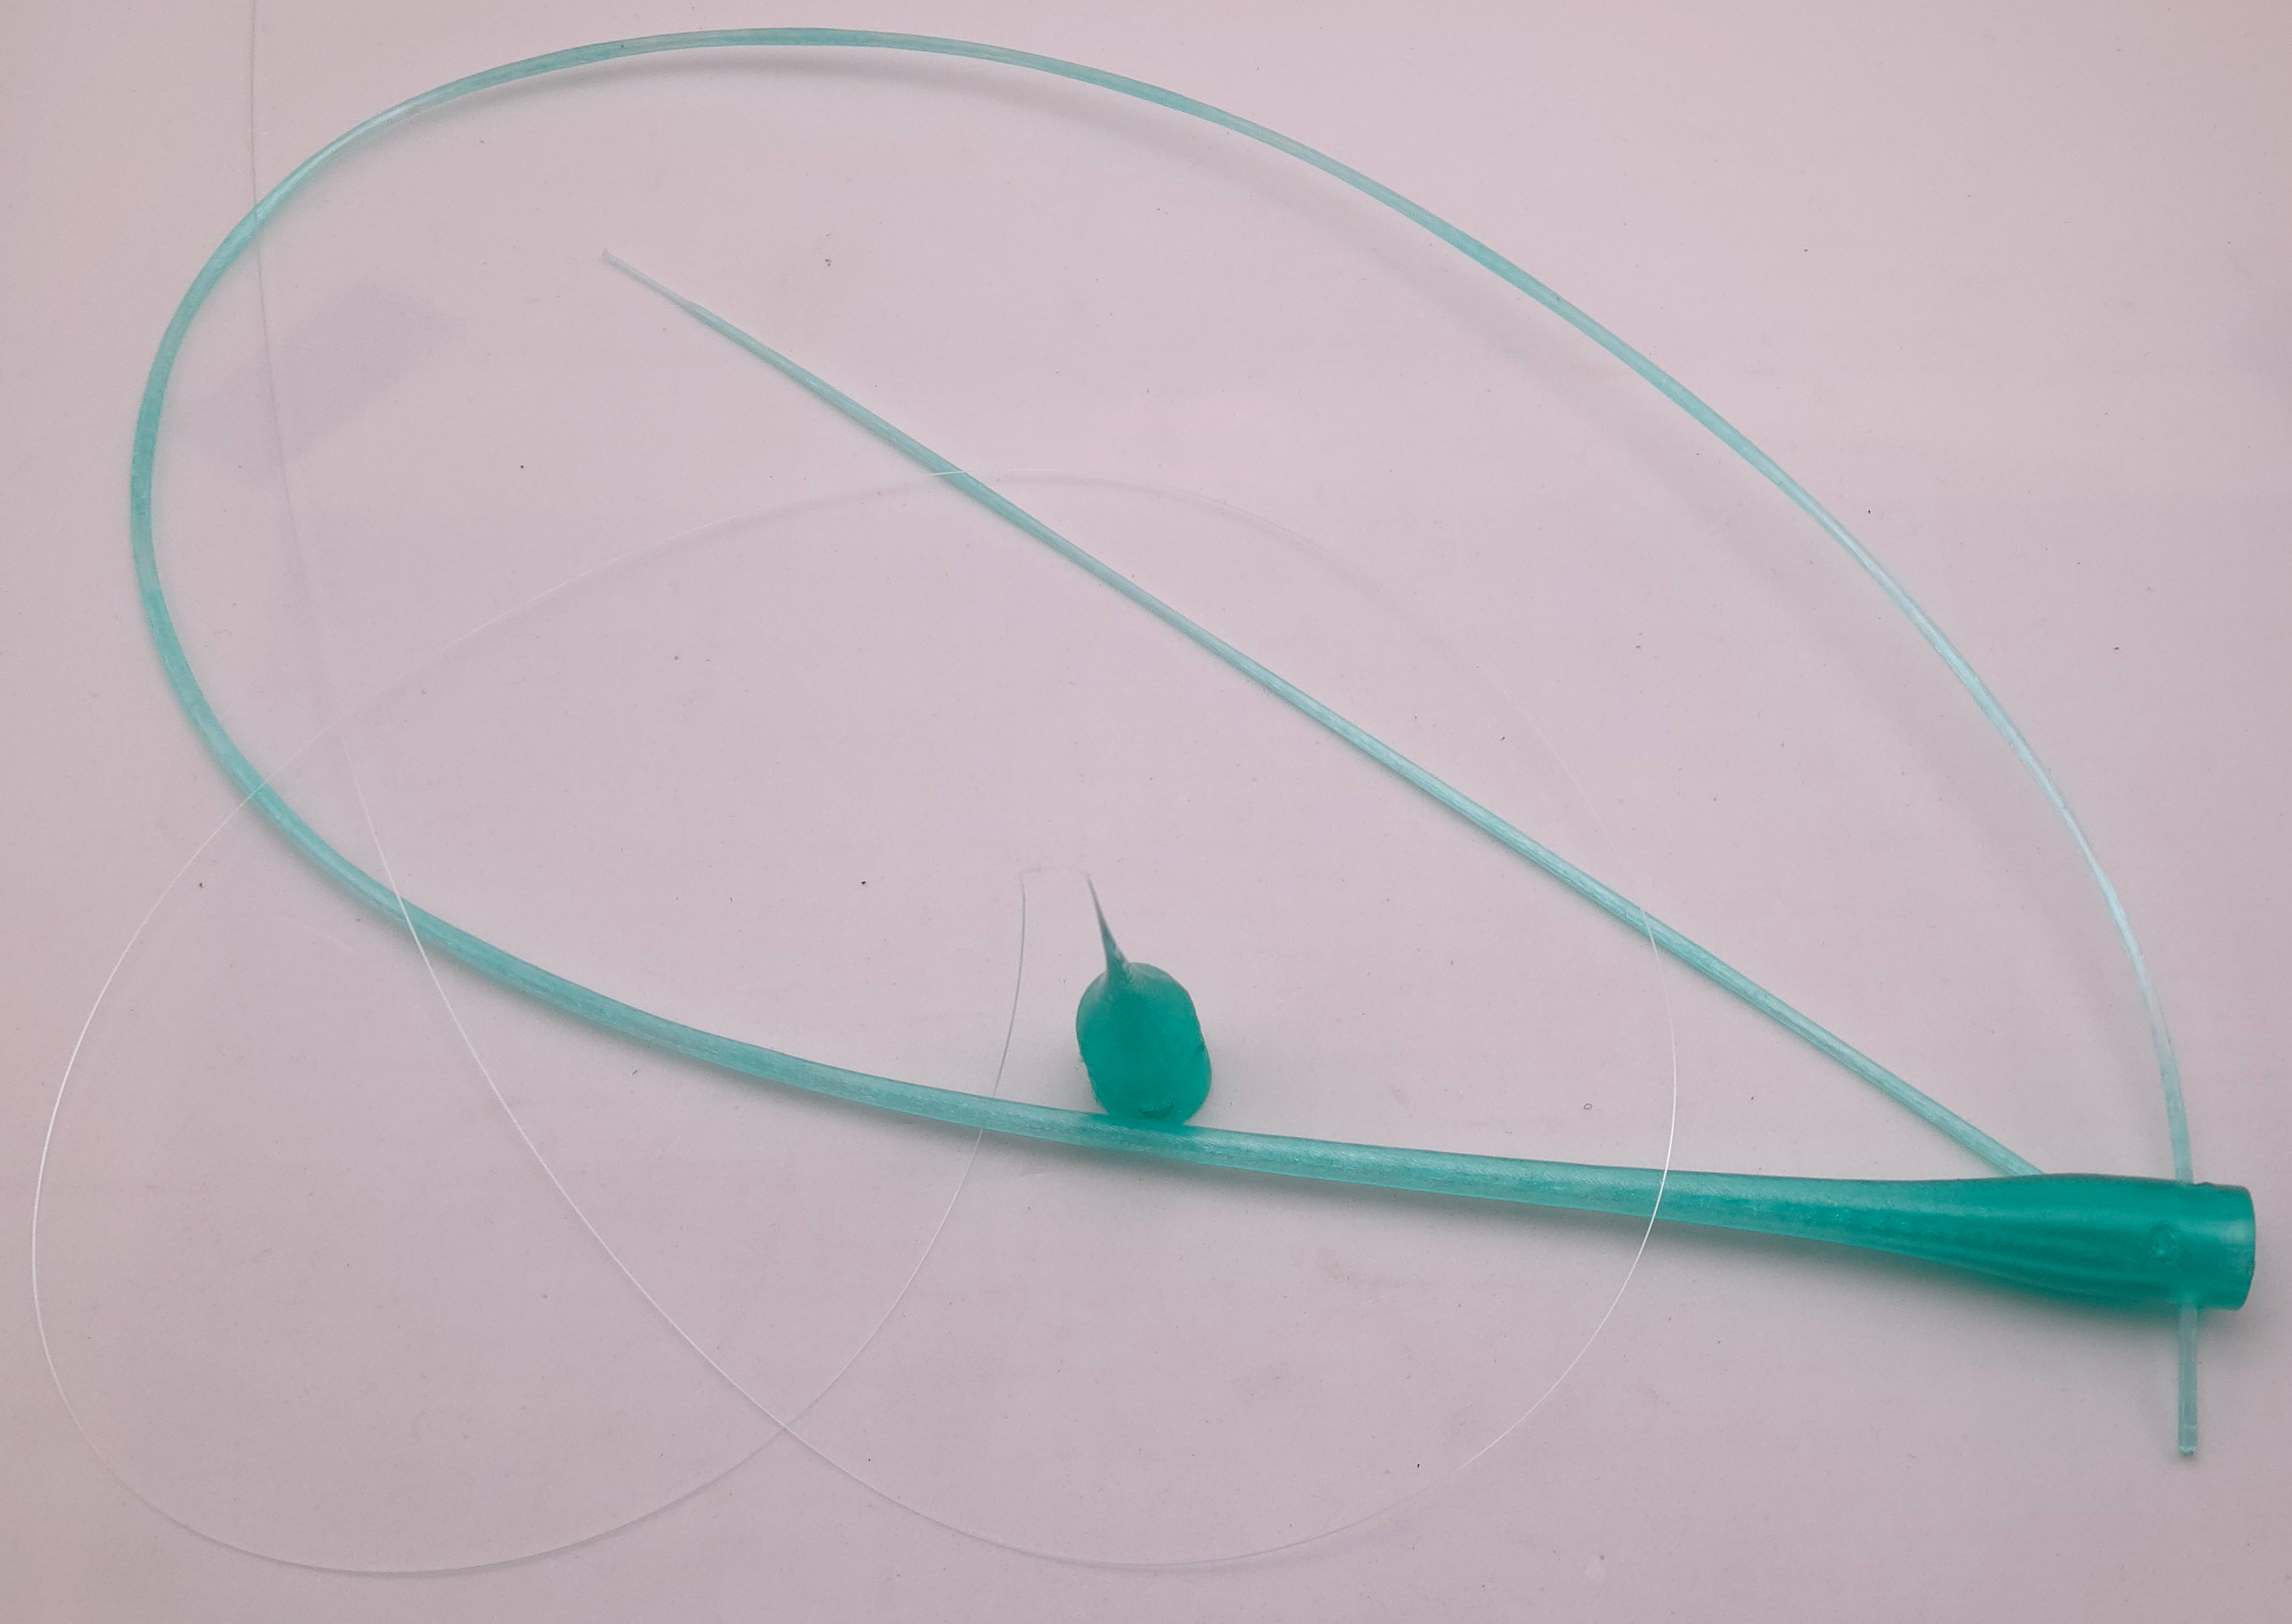
\includegraphics[width=\linewidth]{Sobras.jpg}
    \caption{Preforma restante após o puxamento.}
    \label{fig:sobras}
  \end{subfigure}
  \caption{Resultados do puxamento da fibra \textit{staircase-core}.}
  \label{fig:resultados_multfig}
\end{figure}

\begin{figure}[H]
  \centering
  \begin{subfigure}[t]{0.32\linewidth}
    \centering
    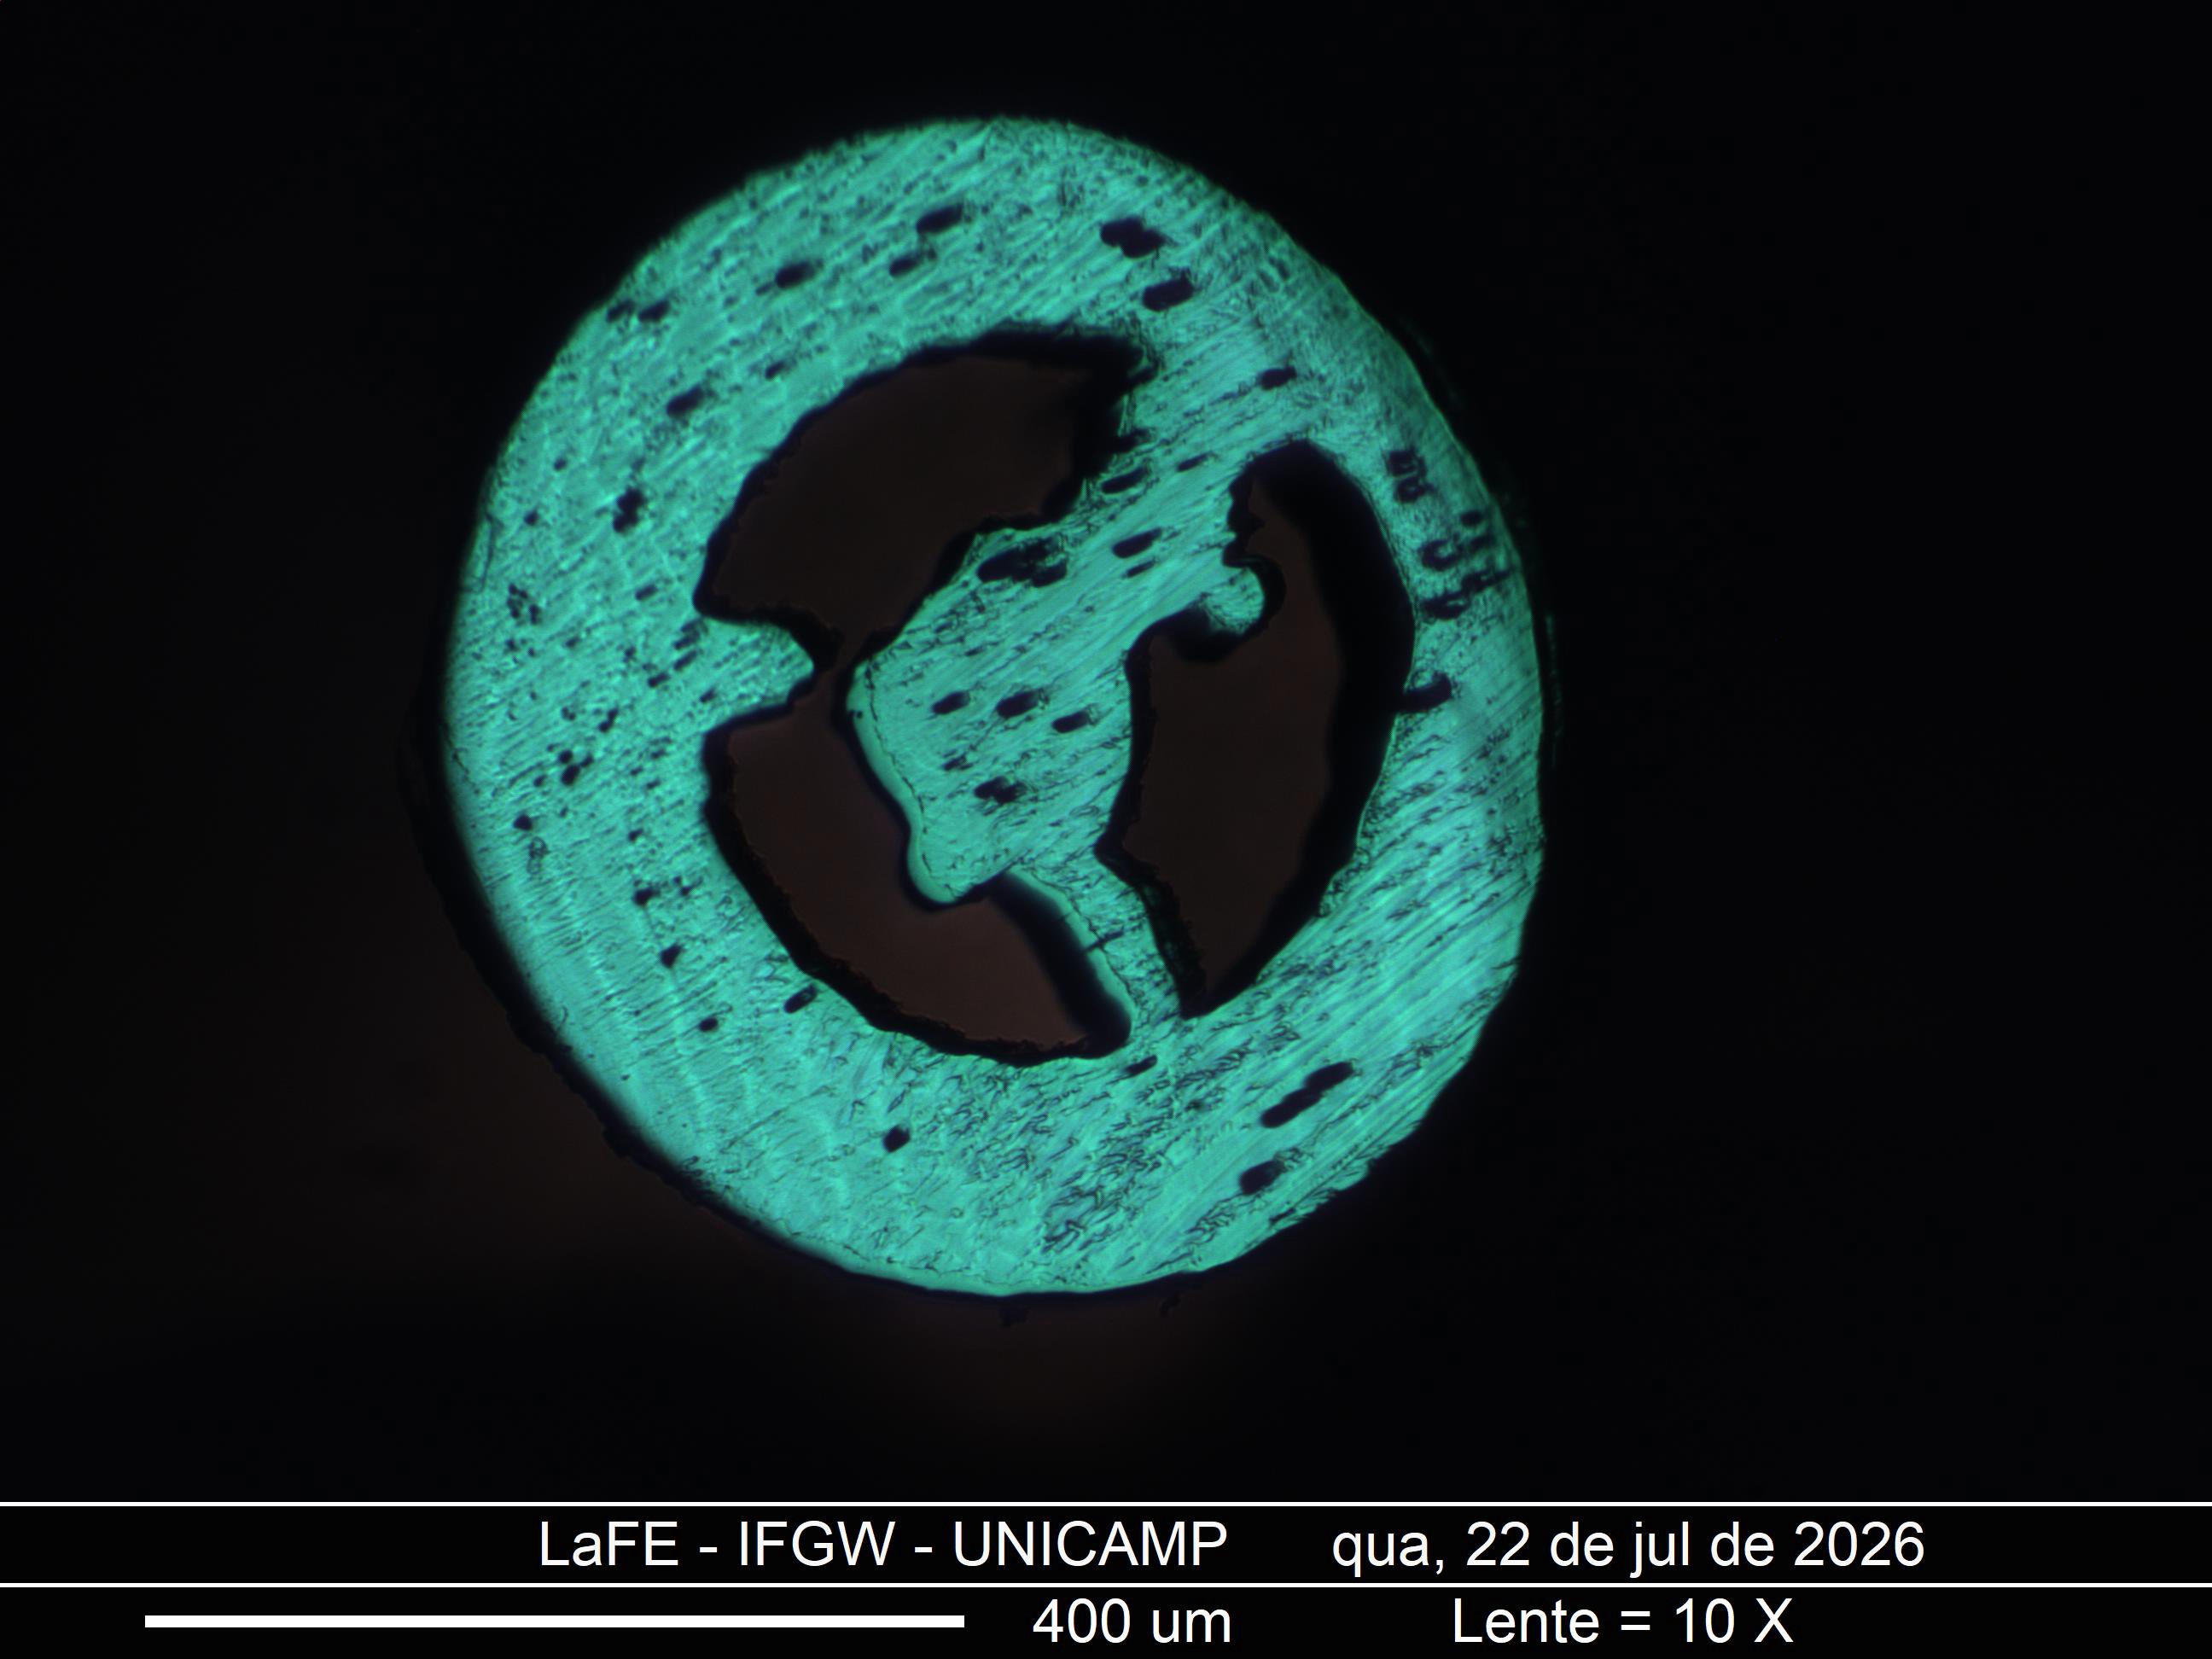
\includegraphics[width=\linewidth]{Banda_A.png}
    \caption{Banda A.}
    \label{fig:banda_A}
  \end{subfigure}
  \begin{subfigure}[t]{0.32\linewidth}
    \centering
    
\includegraphics[width=\linewidth]{Banda_B.png}
    \caption{Banda B.}
    \label{fig:banda_B}
  \end{subfigure}
  \begin{subfigure}[t]{0.32\linewidth}
    \centering
    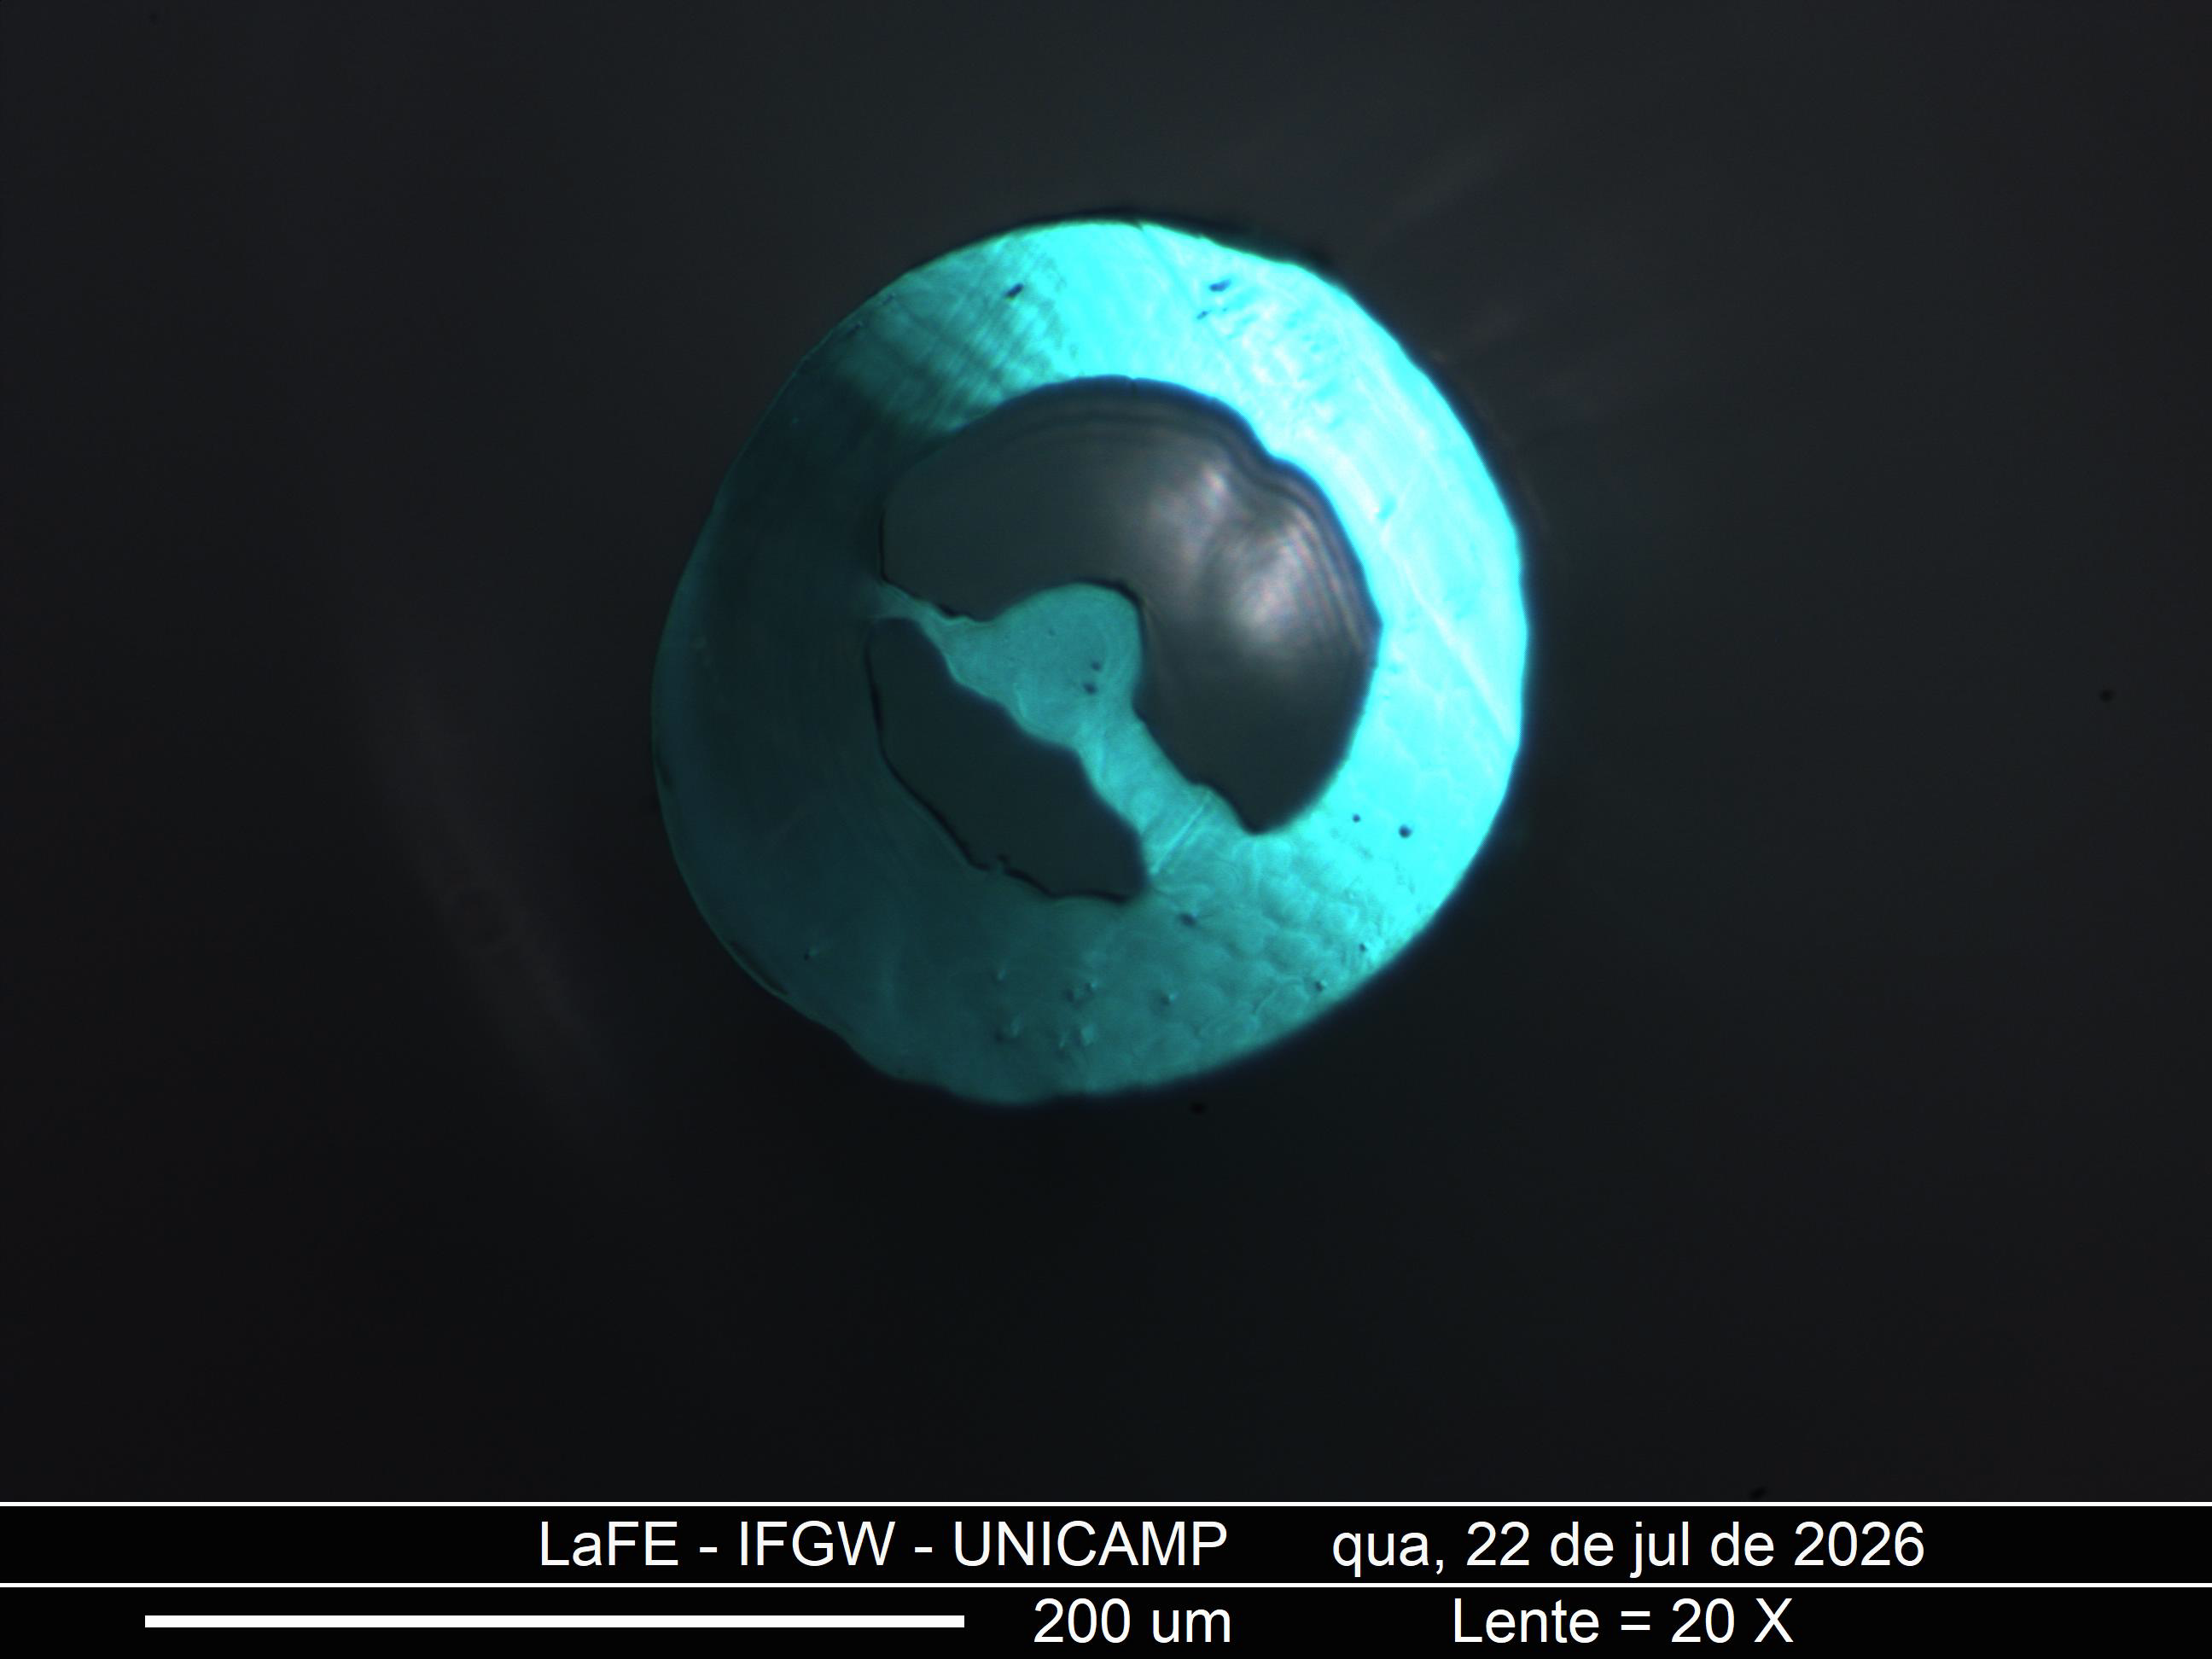
\includegraphics[width=\linewidth]{Banda_C.png}
    \caption{Banda C.}
    \label{fig:banda_C}
  \end{subfigure}
  \caption{Micrografias das bandas produzidas. Cada micrografia foi realizada com uma seção do final da banda.}
  \label{fig:micrografias}
\end{figure}

  \begin{table}[H]
    \centering
	  \begin{tabular}{cccc}	
		  \textbf{Medida} & \textbf{Banda A} & \textbf{Banda B} & \textbf{Banda C}\\ 
		  \hline
      $\phi_{out}$ [$\mu$m] & 567 & 278 & 216 \\
		  $L_{clad}$ & 0.188 & 0.204 & 0.232 \\
      $\phi_{core}$ & 0.232 & 0.242 & 0.182 \\
		  $L_{strut}$ & 0.096 & 0.099 & 0.069
	  \end{tabular}
	  \caption{Medidas relativas e diâmetro externo absoluto na fibra produzida.}
	  \label{tab:medidas_produzidas}
  \end{table}


  \begin{figure}[H]
    \centering
    
\includegraphics[width=0.9\linewidth]{Diametro.png}
    \caption{Gráfico de diâmetro ao longo do puxamento.}
    \label{fig:diametros}
  \end{figure}

\end{document}
